\chapter{Tension on Bolts}
\section{Nomenclature}
\begin{tabular}[t]{lp{8cm}}
		$ [F_{cb}] $ & tension force at failure of common bolt, $ N $\\
		$ [F_{sb}] $ & tension force at failure of steel bolt, $ N $\\
		$ [\sigma_{cb}] $ & tension at failure of common bolt, $ MPa $\\
		$ [\sigma_{sb}] $ & tension at failure of steel bolt, $ MPa $\\
		$ d $ & nominal diameter of M8 bolt, $ mm $\\
		$ F_c $ & tension force of hydraulic cylinder\\
		$ F_{cb} $ & tension force at failure of common bolt, $ N $\\
		$ F_{sb} $ & tension force at failure of steel bolt, $ N $\\
\end{tabular}

\section{Purpose}
Provide basic knowledge on conducting experiment regarding ultimate strength of materials

\section{Safety Procedures}
Close the machine door before every operation.

\section{Conduct Experiment}
\begin{table}[ht]
	\centering
	\begin{tabular}{|c|p{2.5cm}|p{2.5cm}|}
		\hline
		\multirow{2}{*}{No.} & \multicolumn{2}{l|}{Experiment with $d=8\unit{mm}$} \\ \cline{2-3} 
		& $F_{sb}$         & $F_{cb}$                 \\ \hline
		1                    & 33898            & 37377                           \\ \hline
		2                    & 33574            & 37053                           \\ \hline
		3                    & 34211            & 36426                           \\ \hline
		4                    & 33727            & 37053                           \\ \hline
		5                    & 34211            & 36426                           \\ \hline
		Average              & 33323.4          & 36867                           \\ \hline
	\end{tabular}
	\caption{Tension force at failure of common and steel bolts}
\end{table}

\section{Data graphs}
\begin{figure}[ht]
	\centering
	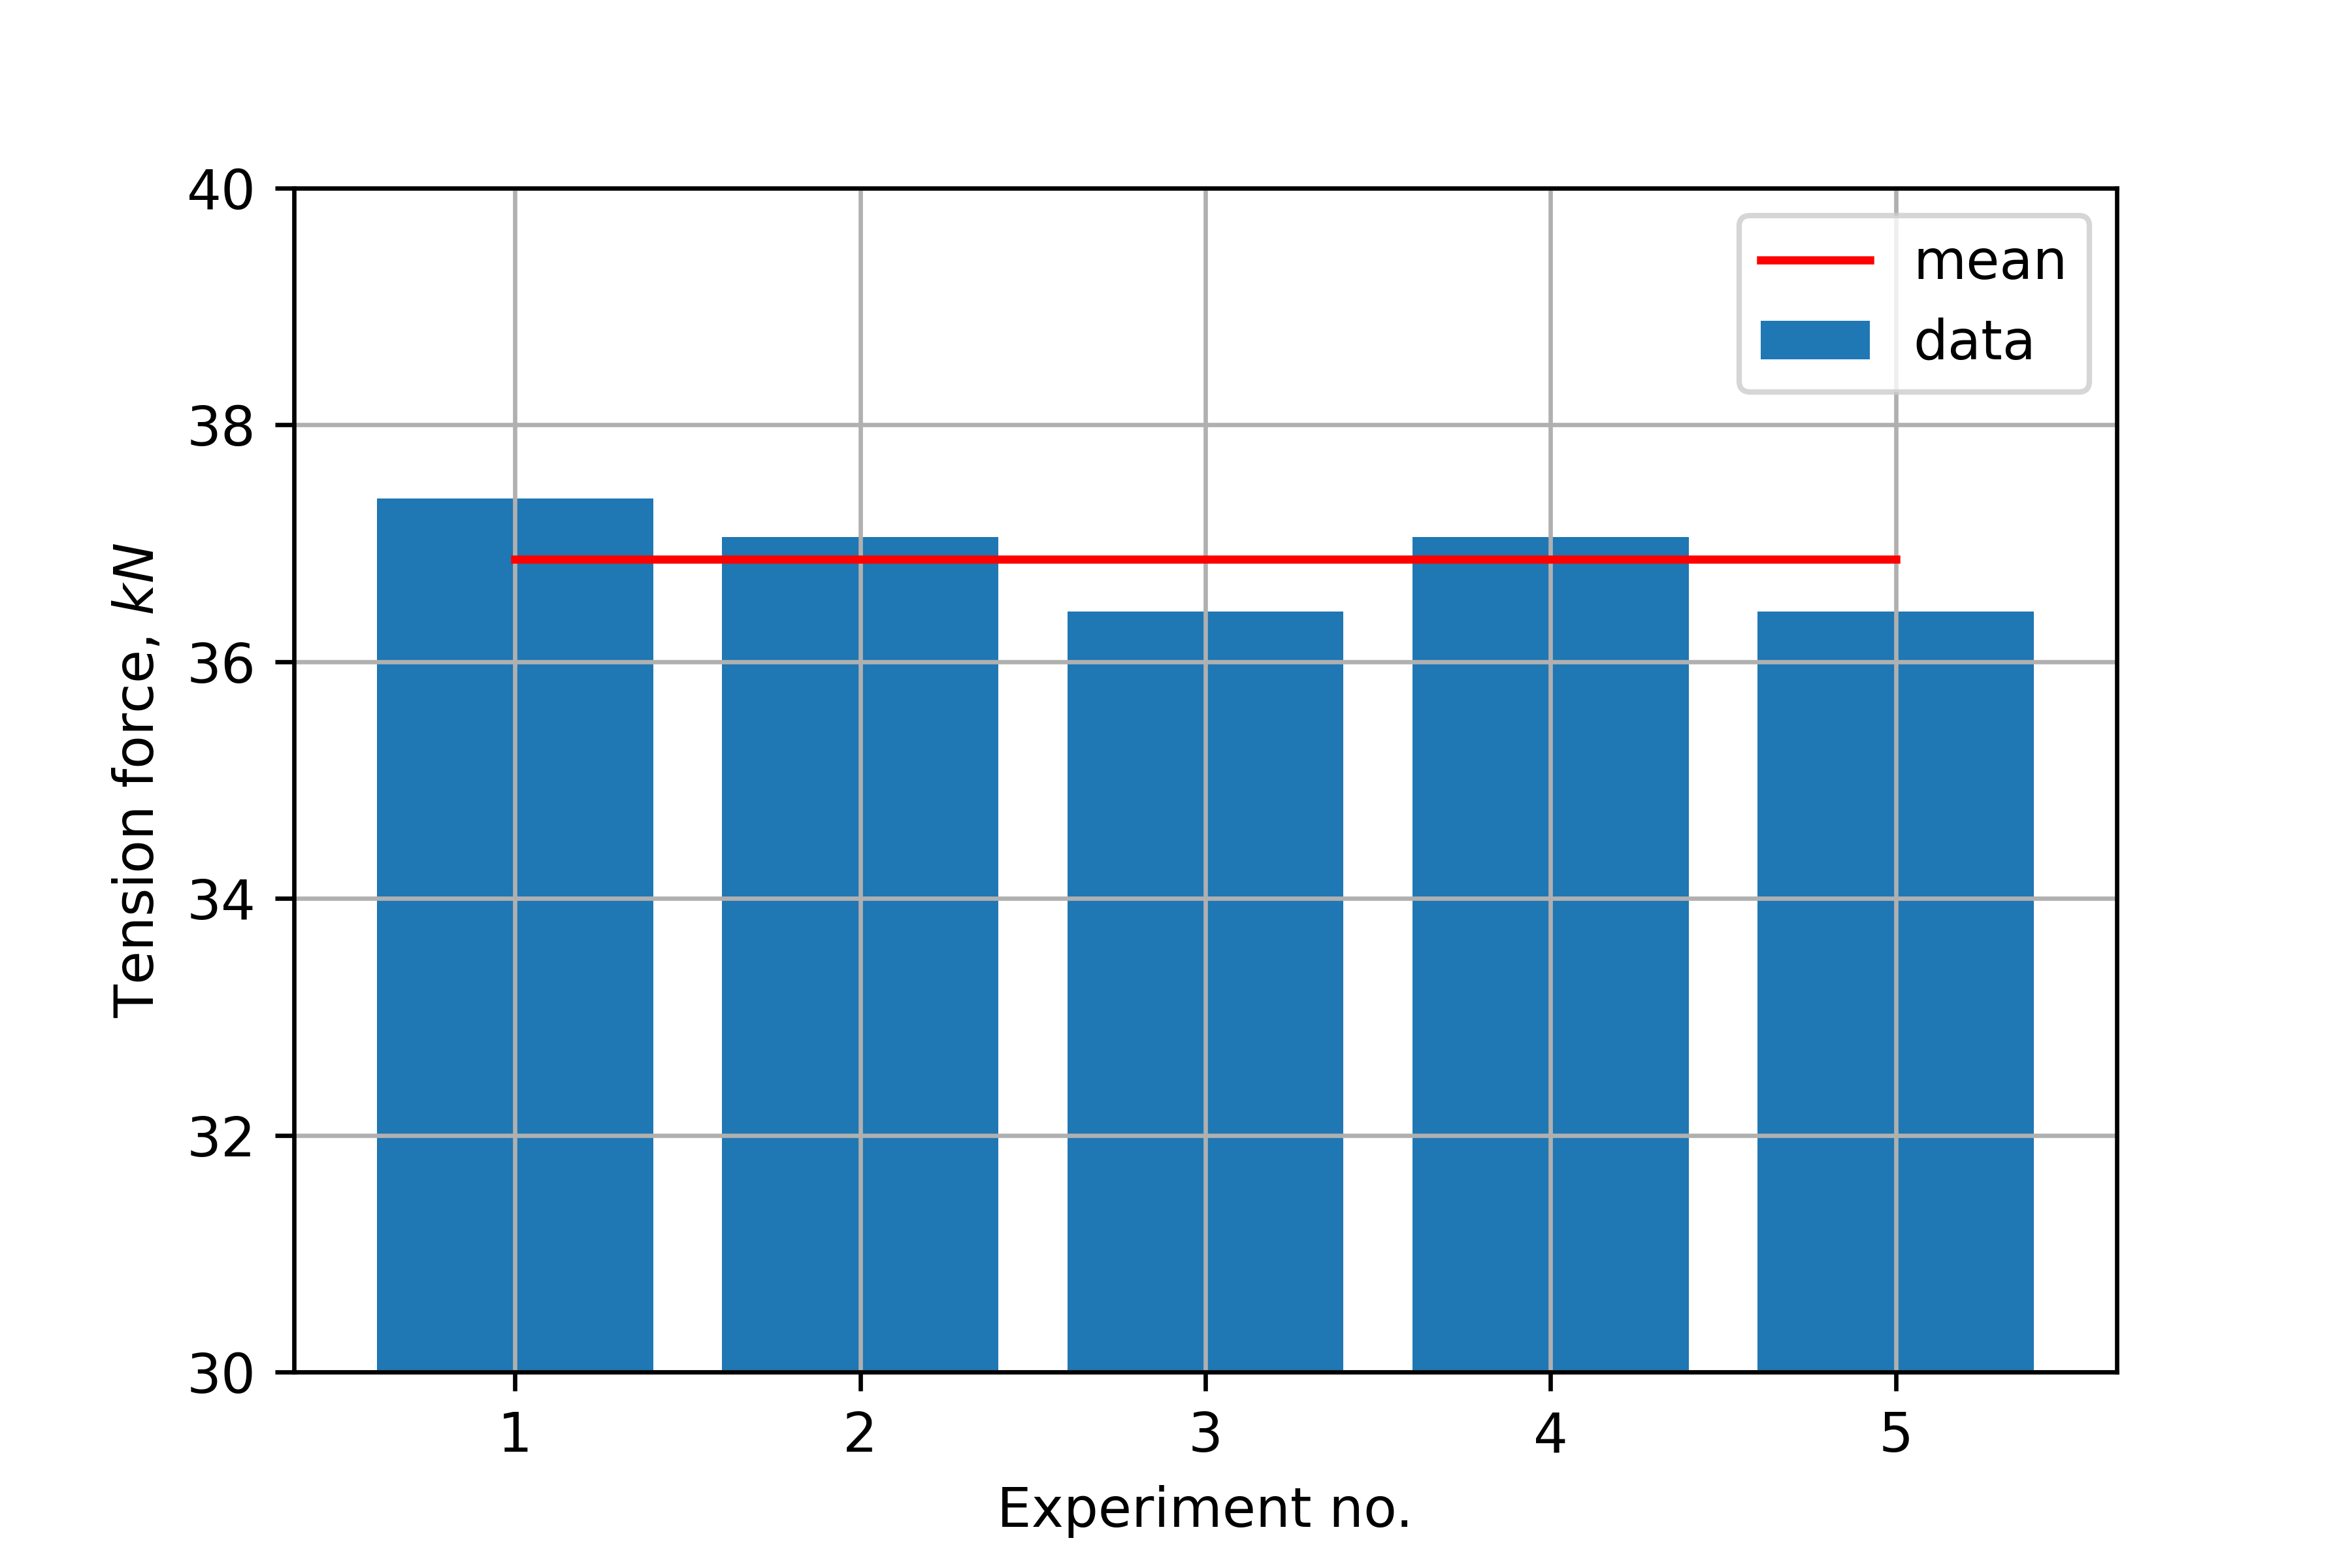
\includegraphics[width=150mm]{Exp2cb.png}
	\caption{Tension force at failure of common bolt}
\end{figure}$ $
\begin{figure}[ht]
	\centering
	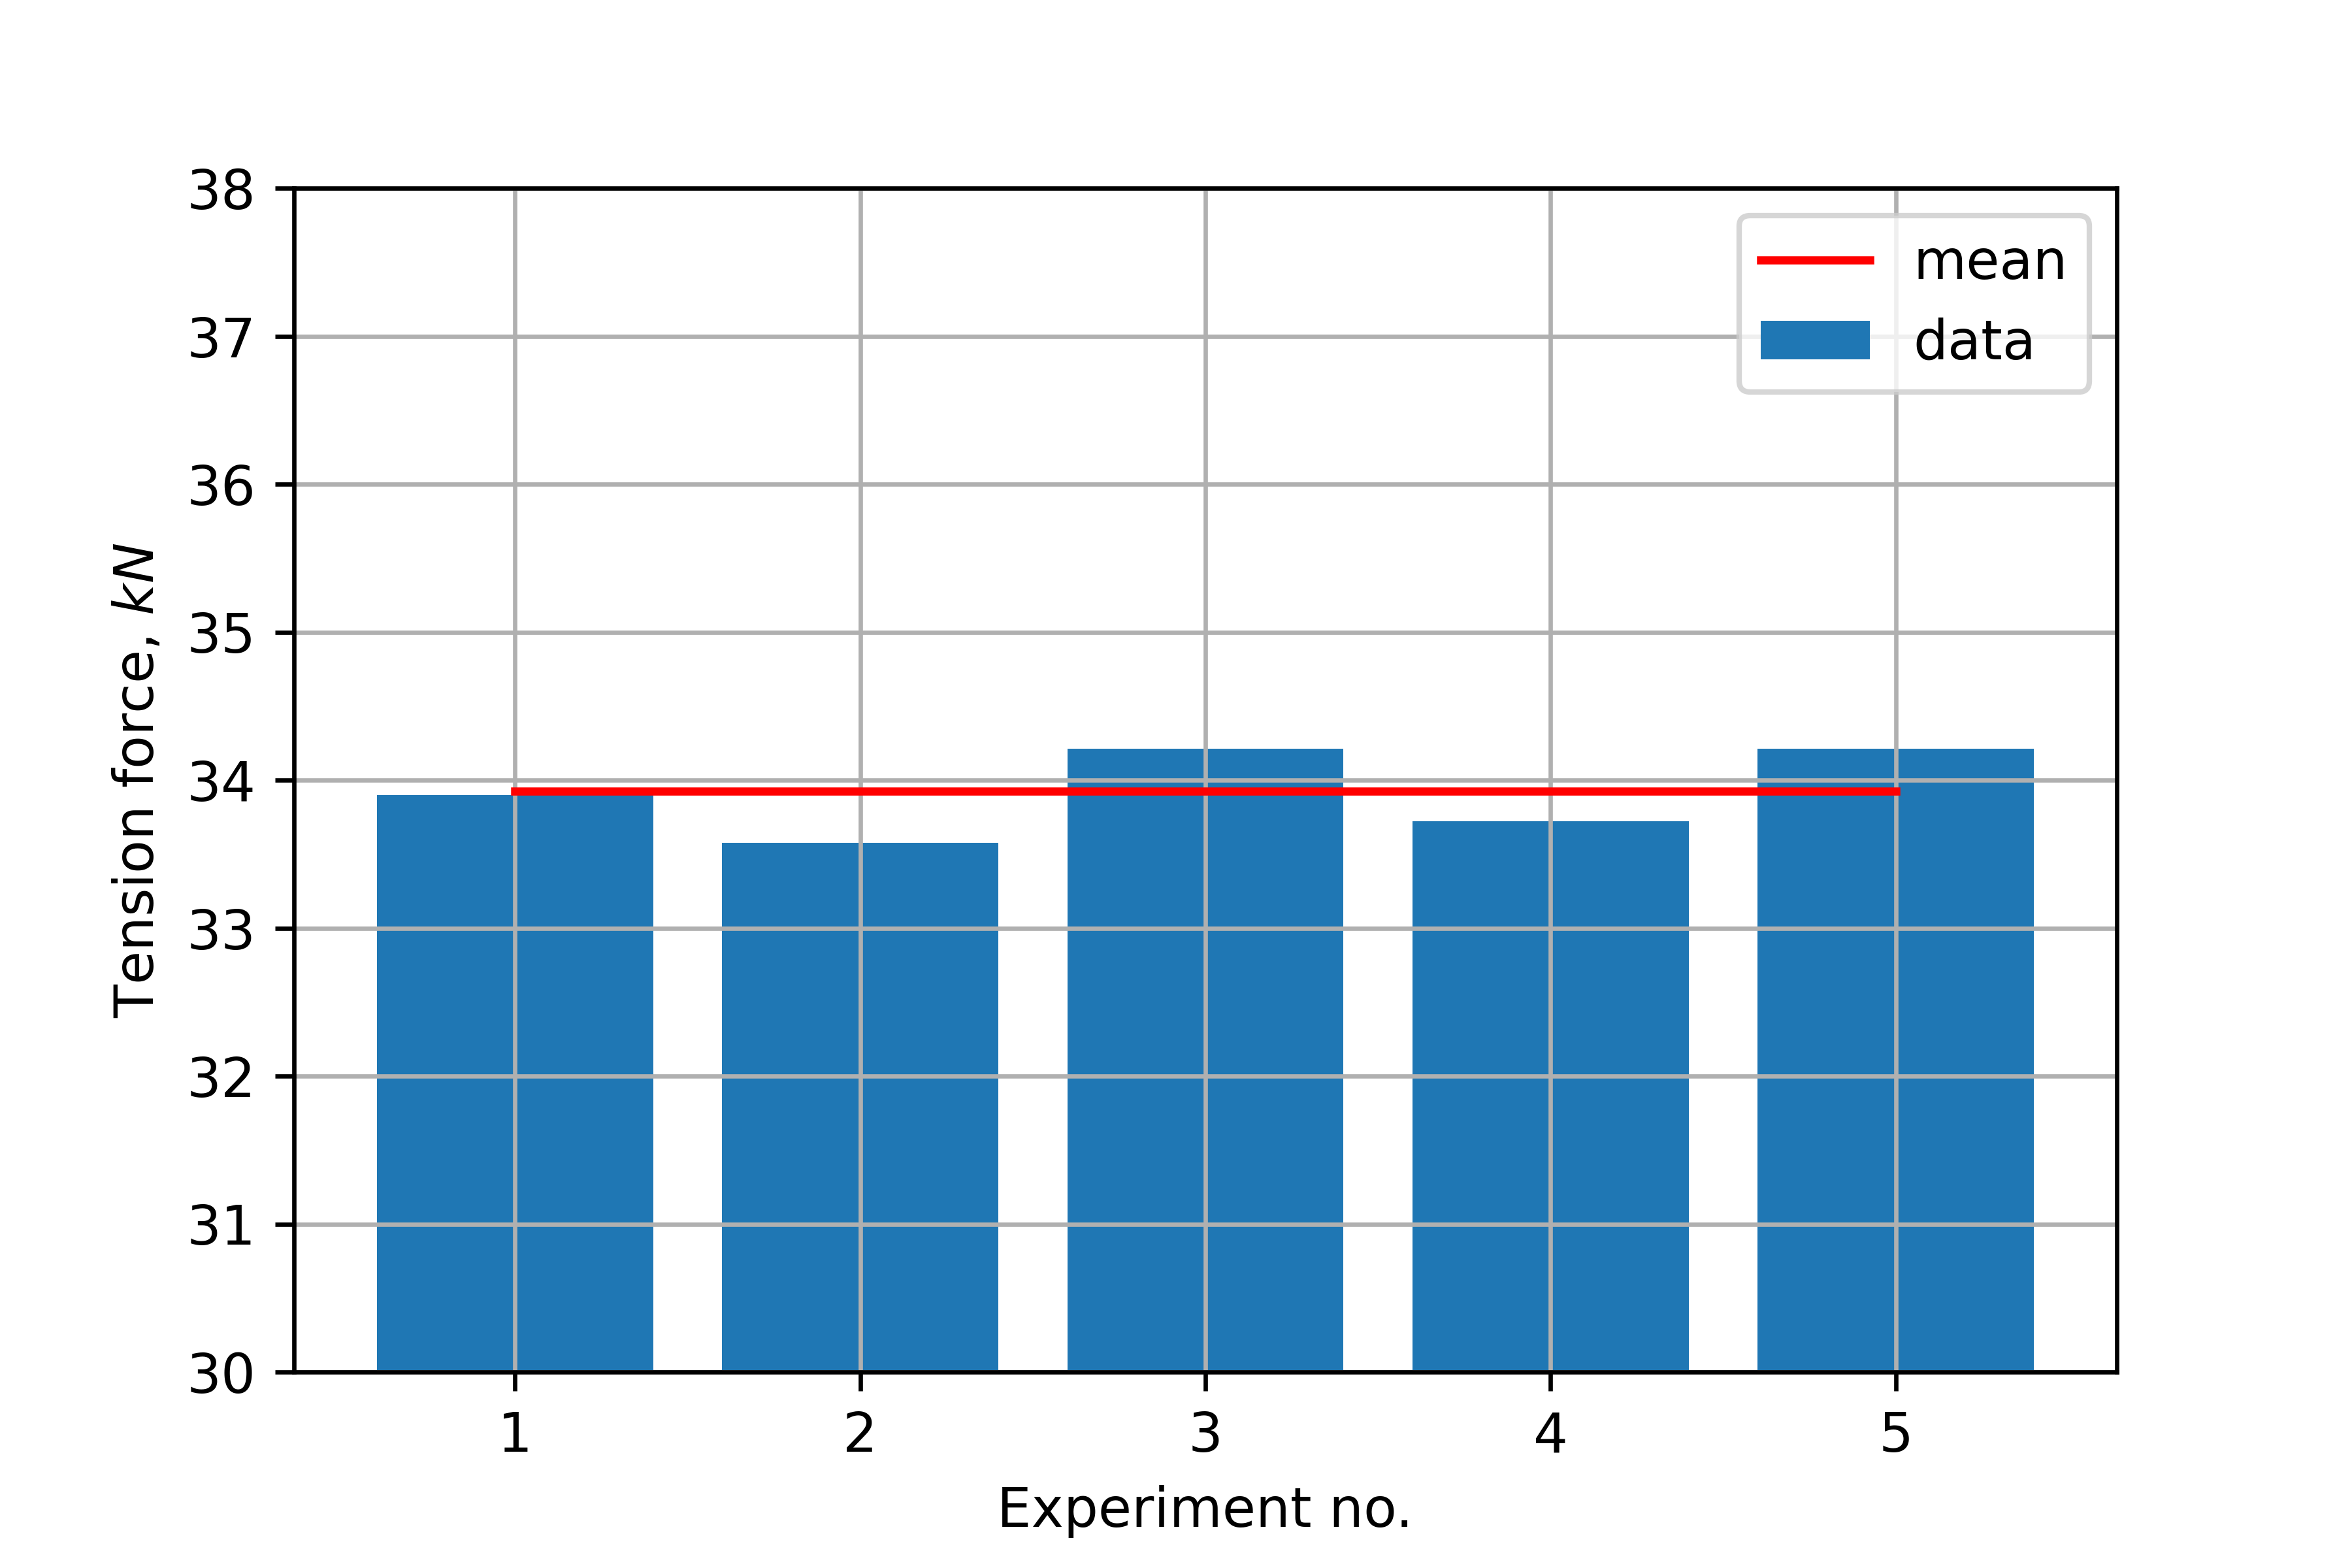
\includegraphics[width=150mm]{Exp2sb.png}
	\caption{Tension force at failure of steel bolt}
\end{figure}